\documentclass{article}

% if you need to pass options to natbib, use, e.g.:
% \PassOptionsToPackage{numbers, compress}{natbib}
% before loading nips_2016
%
% to avoid loading the natbib package, add option nonatbib:
% \usepackage[nonatbib]{nips_2016}

%\usepackage{nips_2016}

% to compile a camera-ready version, add the [final] option, e.g.:
\usepackage[final]{nips_2016}
\usepackage{graphicx}
\usepackage[utf8]{inputenc} % allow utf-8 input
\usepackage[T1]{fontenc}    % use 8-bit T1 fonts
\usepackage{hyperref}       % hyperlinks
\usepackage{url}            % simple URL typesetting
\usepackage{booktabs}       % professional-quality tables
\usepackage{amsfonts}       % blackboard math symbols
\usepackage{nicefrac}       % compact symbols for 1/2, etc.
\usepackage{microtype}      % microtypography
\usepackage{xcolor}
\newcommand\todo[1]{\textcolor{red}{#1}}
\renewcommand\todo[1]{}

\title{Effective assault detection using machine learning and simple arduino sensors}

% The \author macro works with any number of authors. There are two
% commands used to separate the names and addresses of multiple
% authors: \And and \AND.
%
% Using \And between authors leaves it to LaTeX to determine where to
% break the lines. Using \AND forces a line break at that point. So,
% if LaTeX puts 3 of 4 authors names on the first line, and the last
% on the second line, try using \AND instead of \And before the third
% author name.
\author{
  Noah Hollmann \\
  ETH Zürich\\
  Switzerland, Zürich 8057 \\
  \texttt{noahho@student.ethz.ch} \\
  \And
  Supervisor: YunTao Wang \\
  Global Innovation Exchange, Tsinghua University \\
  China, Beijing \\
  \texttt{yuntaowang@tsinghua.edu.cn} \\
}

\begin{document}
% \nipsfinalcopy is no longer used

\maketitle

\begin{abstract}
  Detecting special breathing patterns in a sequence of breathing can have many applications. In this paper the focus is on detecting a special SOS pattern. For this purpose a method to collect data and to train a model is described. In order to simplify the data it is segmented and then clustered into groups. Then a Hidden Markov Model is trained to detect sequences of these group numbers. The paper provides all the neccessary details to train such a model effectively.
\end{abstract}

\section{Introduction}
\label{sec: introduction}
A device to detect if a person is being attacked could have a great impact for the security of people worldwide. The problem of women being assaulted is global. In India alone there were 24,923 rape cases reported in 2012 \footnote{ National Crimes Record Bureau, Crime in India 2012 - Statistics Government of India (May 2013)}, while the number of unreported rape cases is estimated to be much higher. In the same year the gang rape of a 23-year-old student on a public bus, on 16 December 2012, sparked large protests across the capital Delhi. \footnote{ "Video: Protests grow over gang rape of Indian woman". London: Telegraph. 19 December 2012. Retrieved 21 December 2012.}. In the US the problem is especially prominent on university campuses and is currently highly discussed. The fear of an assault should not be underestimated as well, it affects the lives of people in everyday life. \\
We built a prototype of a device, that can detect an assault, even when the victim is not able to actively use a device. This is done by recognizing special "SOS" breathing patterns. For this task the device is equipped with a stretch sensor around the chest. I built a machine learning algorithm that in its core trains a hidden Markov Model to recognize these special patterns and also incorporates One-Class classification using the Gaussian Normal Distribution.}\\
Even when the data collection device is strongly optimized the data collected still has many problems. The low price of the stretch sensor has some trade offs: The stretch-data has a very limited range (about 30 steps) from the lowest to the highest stretch and it "remembers" a strong stretch. Also moving of the body affects the stretch, the sampling rate is not constant and the test data is limited since it is collected as part of this project. To make things worse it is important that the algorithm has a very high accuracy, especially false detections must be very unlikely. This makes the task to design an algorithm very difficult. This explains why there is almost no research regarding the analysis of the breath using machine learning.\\
The proposed algorithm goes through four phases. First a sequence is divided into segments at changepoints (the mean of these segments changes). Next each segment is approximated by a polynomial. These polynomial are clustered using the k-means algorithm. Finally a HMM (Hidden Markov Model) is trained onto the sequence of clusters of the collected patterns. Additionally the mean of the number of segments in the pattern and the length of the pattern are saved. The approach works very well for the proposed pattern to be detected, however not all patterns can be trained using this approach. Patterns with variable length (variable parts in pattern) would need to disable comparing the lengths. Long patterns are restricted by the number of states of the HMM, recurrent neural networks could train longer sequences, Also some patterns can not be trained because they are too similar to normal breathing or the used device can not adequately record the breathing.
\section{Related work}
\label{sec: related}
There has been some previous research in recognizing patterns in time-series analysis based on the same core method used in this algorithm. \cite{TimeseriesSri, BenChoi, FindingP10} This work proposed the same approach of dividing at changepoints, clustering and then training an HMM.\\
The problem of speech recognition is related to this problem and most importantly a very well studied field. While newer approaches focus on RNNs \cite{machine-learning-paradigms-for-speech-recognition-an-overview} because they can detect longer sequences, some other approaches use HMMs \cite{machine-learning-paradigms-for-speech-recognition-an-overview, zhangSpe91}. Because the sequences the algorithm is supposed to detected will not be very long it is not necessary to train an RNN, an HMM will be more effective for our proposed problem.\\
The big amount of noise of the sensor requires some preprocessing of the data. MATLAB provides great help for this and \cite{JSSv033i05} provides great help for choosing the correct methods. \\
The previous work of Zehao Sun, et al. \cite{Sun2015} has used another approach to detect assaults, which I also looked into. They simply use the accelerometer of a smartphone without any active signal being sent by the victim. In their approach they have proposed the idea of looking at features measuring the strength of acceleration as well as irregularity of the motion. They use a shared two-class classifier in combination with an individually trained one-class anomaly detection system. We seek to improve this research with our custom device setup and an improved approach regarding the machine learning.\\
\section{Data collection}
\begin{figure}[h]
  \centering
  \fbox{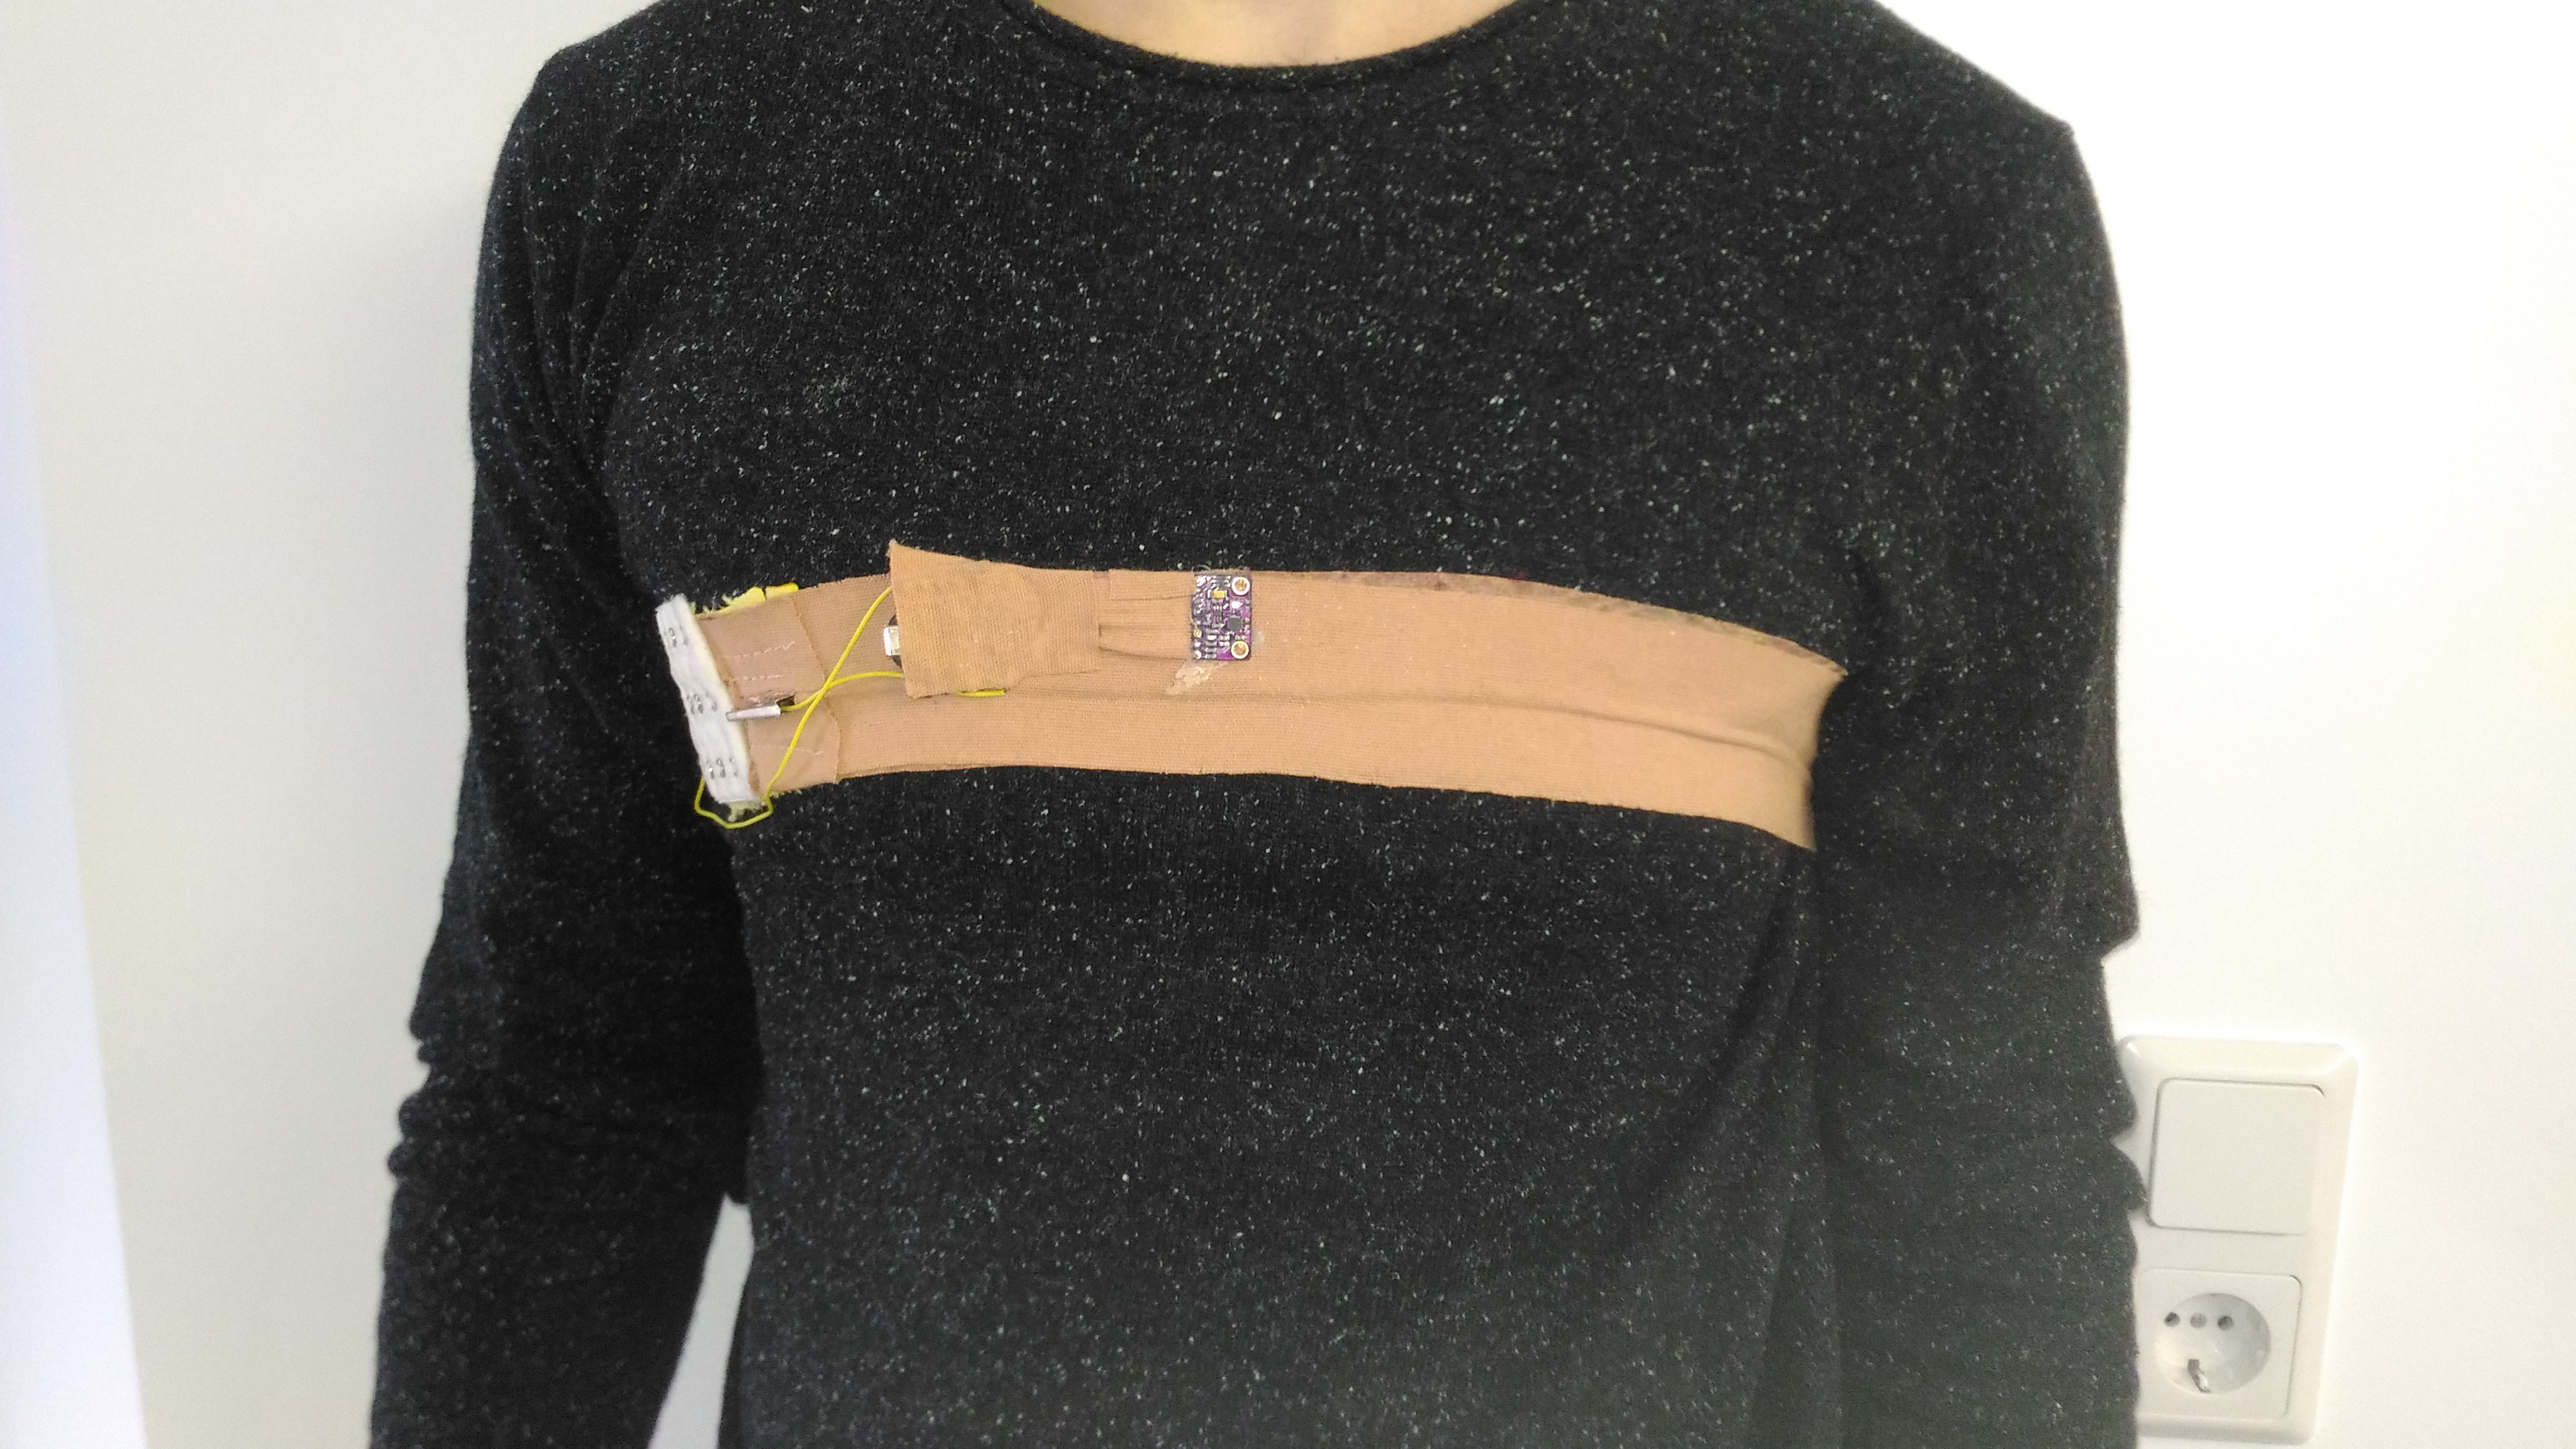
\includegraphics[width=6cm\textwidth]{sensorImg}}
  \caption{The developed sensor in use}
\end{figure}
\label{sec: collection}
\subsection{Device setup}
The proposed prototype is a stretchable band that can strapped around the chest. Inside the band there is a stretch sensor, also an accelerometer is placed on the front of the chest. A battery and a Bluno Arduino chip is placed on the right side of the body. Bluno Arduino provides BLE 4.0, which is a more energy efficient way to send Bluetooth data, almost all modern smartphones support BLE 4.0. Running on the chip is a program that encodes data from the accelerometer as well as the stretch sensor and sends it over Bluetooth.
[Bilder device]
\subsection{Phone setup}
To collect the test data, I developed an Android app that decodes the data and saves it to the SD Card. Using the GUI the app can also save a number for every saved data point. This way the patterns can be flagged and separated from the normal breathing.
\subsection{Pattern proposal}
For an optimal pattern it is important, that it differs quite strongly from normal breathing and that the sensors are able to record it adequately. \\
In normal breathing, the rate of the breath is constant, the strength of the breath is not maximal, the breath is never stopped and breathing in and out always alternate. Our pattern should break all these rules. \\
The chest is only inflated when breathing in is coming close to the maximum. Only the inflation of the chest can be detected. Holding the breath at a low level of chest inflation can not be detected, since it is equal to breathing with a low amount of air in the chest. \\
The proposed pattern is the following, executed in about 5 seconds: Deep breath in, stop - Deep breath in - Deep breath out - Deep breath in, stop, Deep breath in, stop, Deep breath in - Deep breath out \\
\subsection{Automatic data generation}
Since it is very labour intensive to collect many instances of this pattern, I developed a way to generate more test from the previously collected ones. First the test data is distorted in many ways. Breathing might be executed in different speeds and with different strengths. Also some noise is added that simulates movements of the arms, I tried to synthesize the noise that is found in practice. Noise is usually at zero, but some areas have strong noise added to it. Using this synthesized data the algorithm can be trained and tested more robustly. Figure 2 shows an example of artificially generated data.\\
\begin{figure}[h]
  \centering
  \fbox{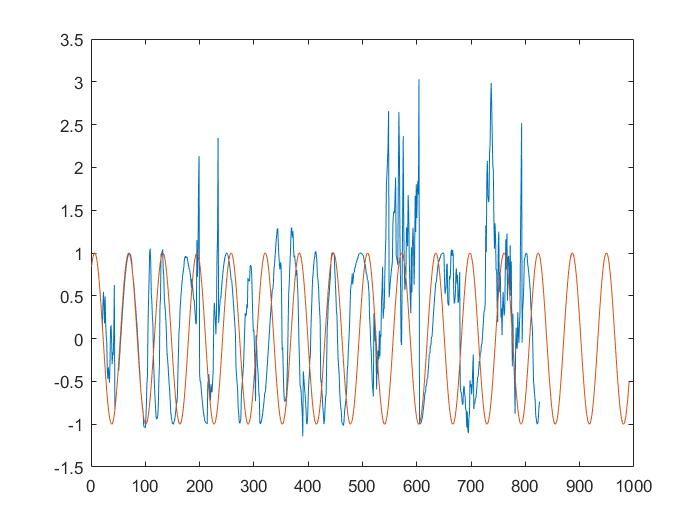
\includegraphics[width=8cm\textwidth]{genData}}
  \caption{The blue curve shows the generated data, the orange curve shows the original}
\end{figure}
\section{Training}
\label{method}
In this section I describe my method for learning from past observable data. The proposed algorithm consists of major steps. First a sequence is divided into segments at changepoints (the mean of these segments changes). Next each segment is approximated by a polynomial. These polynomial are clustered using the k-means algorithm. Finally a HMM (Hidden Markov Model) is trained onto the sequence of clusters of the collected patterns. Additionally the mean of the number of segments in the pattern and the length of the pattern are saved.
\subsection{Preprocessing}
Because of the strong noise in the original data, which strongly fluctuates between close values, the data is smoothed first. Then, in order to eliminate the different breathing strength of different persons, the device is calibrated to the range of the persons breath and the data is normalized from 0 to 1 within this range.
\subsection{Changepoint detection}
The sequence should be divided into segments that can be interpolated well by the approximation in step two. They should be split, where there is a major change in the data, not be too short and have a fairly similar size. MATLAB provides the function findchangepts. This method can be used to find changepoints in the mean value, which works best for our pattern. It is similar to the method proposed by Ben Choi and Taylor \cite{BenChoi, Taylor}.
\subsection{Segment approximation & Featurization}
Each segment needs to be featurized for clustering, this is done by approximating each segment and adding some features. The segments can be approximated in many ways as described in "MATLAB for Data Analysis" \cite{dataanal37}. For different patterns, there can be different solutions to this problem, our patterns can be described by polynomials very well. Because different persons wearing the device will stretch the sensor differently in the resting state, the starting value of a segment should not be included in the features of it, making it more independent from the mean stretch. \\
An important metric for the segments is their length, which is not included in the polynomial describing it, as well as the difference in the stretch before and after the segment. Those two important metrics are added as features to each segment. Thus the feature vector consists of the factors of the polynomial describing each segment, excluding the constant factor, as well as length and change. \\
\subsection{Clustering}
After describing all the segments, we partition them into groups by clustering. MATLAB implements k-means clustering measuring the similarity between segments by the Euclidean distance. However the features contain the factors of the polynomials as well as the length and change of each segment. On average the length is very large compared to the other features and would thus be weighted much stronger by the algorithm. To avoid this we limit each feature by a logistic function. We set the steepness of the curve for each feature, and give a weight to all of them. This way even when features are very large, they tend to stay together and never completely out rule other features. Also the change feature which is more important can be given a higher weight.
\subsection{Training Hidden Markov Model}
After clustering all the segments into groups every instance of a pattern is a sequence of numbers that correspond to a clustered group. In training the model of the HMM I propose my own solution, which strongly differs from the one used by Ben Choi \cite{BenChoi}. The number of the group is treated as an emission of the HMM and the state transitions are left for the HMM to build. Because a shorter sequence a will always have a higher or equal probability than {a, b}, shorter unfinished sequences would always be preferred. In order to avoid this I add a new emission at the end of each sequence that denotes the end of a pattern. Afterwards the HMM is trained for all the sequences of our pattern.
\subsection{One-class Classification}
There are other indicators for a sequence as well. These could be very many like a spectral analysis and many more. In this project I just use the length of a sequence and the number of changepoints (segments) in it. The mean of these two values is saved. Thus a Gaussian distribution can tell how likely these two parameters are for each pattern.
\section{Detection}
In order to detect a pattern, we can do the following. The algorithm stores a list of indices, where possible patterns could start. Whenever data is added, we check if there is a new changepoint. If yes, the new segment is featurized and according to the pretrained cluster centers given a group number. Now the list is used to check if the saved indices are still likely to become a finished pattern, using the Gaussian distribution and the HMM. The likelihood of the HMM is given by calculating the probability of the sequence of groups for this model. If the likelihood is below a threshold, they are disposed from the list. Also if the sum of the probabilities of sequences with higher length or more changepoint is below a threshold, the sequence is exposed as well. This use done using an integral over the Gaussian distribution. If they are above those measures, then it is checked if they are still above the threshold if the finishing group number is added to the end. If this is true, then they are deleted from the list and saved as a detected pattern. Otherwise the next data point is examined.
\section{Evaluation}
\label{experimental}
\begin{figure}[h]
\centering
\begin{minipage}{.48\textwidth}
  \centering
  \fbox{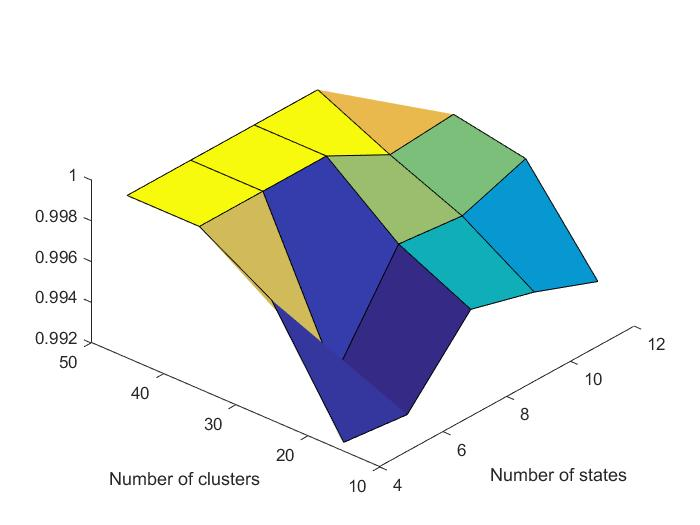
\includegraphics[width=6cm\textwidth]{CorrectDetectionsCLUSTERSvsSTATES}}
  \caption{Correctly detected patterns\\varying No of states and clusters}
  \label{fig:test1}
\end{minipage}%
\begin{minipage}{.48\textwidth}
  \centering
  \fbox{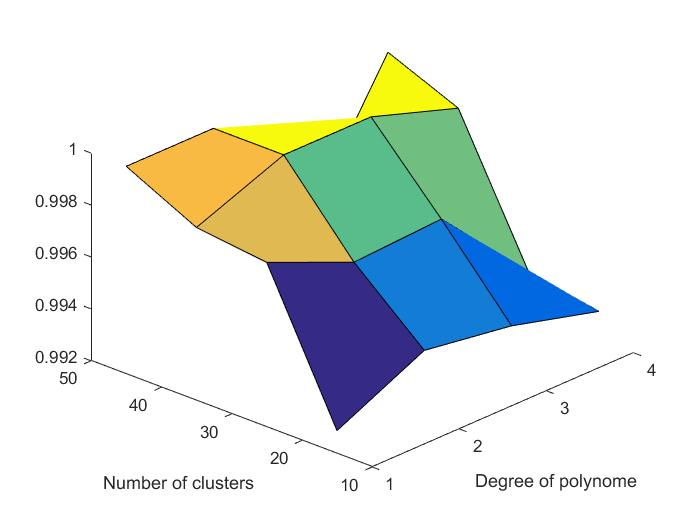
\includegraphics[width=6cm\textwidth]{CorrectDetectionsCLUSTERSvsDEGREE}}
  \caption{Correctly detected patterns \\ varying No of states and clusters}
  \label{fig:test2}
\end{minipage}
\end{figure}
\begin{table}[t]
  \caption{Optimal Parameters for the pattern found by grid search}
  \label{sample-table}
  \centering
  \begin{tabular}{llll}
    \toprule
    Polynome degree     & Polynome degree     & No of states &  Changepoint-method \\
    \midrule
     1  &  15  & 10 &    2 \\
     1  &  25  &   4 &    2 \\
     1  &  25  &   4  &   3  \\
     2  &  15  &  10   &  2  \\
     2  &  25  &  12&     2  \\
     2  &  15  &  10 &    3 \\
     2  &  25  &   6  &   3  \\
     2  &  35  &   8   &  3 \\
     2  &  15  &  10    & 4 \\
     3  &  25  &   4&     2 \\
     3  &  25  &  4  &   3  \\
     3  &  25  &  10  &   3   \\ 
     3  &  15  & 10    & 4    \\
     3  &  25  &  10    & 4     \\
     4  &  15  &  12     &3 \\
     4  &  25  &  12&     3   \\
     4  &  35  &   8 &    3  \\
    \bottomrule
  \end{tabular}
\end{table}
\subsection{Datasets, Metrics and Methodology}
A dataset with initially 150 pattern instances was used for training. After synthesizing more sequences the dataset contained 750 pattern instances. In order to adapt the parameters a dataset with 53  pattern instances were used.  After synthesizing more sequences the dataset contained 265 pattern instances. To test the model a dataset with 50 pattern instances was used.  The dataset was collected for only one person. More data can be collected following the guidelines given in the section Data collection. The dataset was calibrated to a min stretch of 475 and a max stretch of 515.\\
The metrics used to evaluate the accuracy of a model are the percentage of valid patterns in a sequence that were detected by the algorithm and the percentage of detected patterns that are valid. A detected pattern is assumed to be valid, if more than half of the data points in it are part of the correct pattern. Thus a sequence is a valid pattern if the majority is part of the right pattern. If this is given, then the valid pattern that was saved in the dataset is considered to be detected. This can be justified, because we want to give an alarm, if the pattern just occured. This is the case if it is included in the detected patterns. The percentage of detected patterns that are valid has the weakness that the algorithm could detect many sequences for one valud pattern, thus decreasing the effect of one misclassified sample. However the algorithm does not systematically do this, thus the measure is still precise.\\
Using optimized paramters on the parameter dataset, we achieve 0\% erronous detections and detect 89\% of the patterns in the dataset. \\
\subsection{Impact of Model Complexity} \\ 
I used a script to evaluate the accuracy of the model trained with different parameters that describe the model complexity. I created a list of plausible parameters and iterated through all combinations of those. The examined parameters include the number of states, degree of the approximating polynome, the number of clusters and the used changepoint method. Increasing the number of states, polynomes or the degree of the polynome does not seem to have a strong impact on the accuracy of the algorithm, it is rather the combination of the parameters. Table 1 shows the most successful parameter combinations.
\subsection{Impact of Probability Threshold} \\
Different thresh hold for accepting a sequence as detected have been tried. Using grid search the optimal parameter for the log likelihood of the HMM was found to be -35, for the Gaussian distribution it was found to be -60. With these parameters it can also be fine tuned after training, if there are too many false detections or too few correct detections.
\medskip

\small
\bibliographystyle{unsrt}
\bibliography{mybib}

\end{document}